\chapter{Custom EIT Meshes}
\label{chap:chapter-5}

\emph{This work has been presented in part at: 
 the 21st International Conference on Biomedical 
 Applications of Electrical Impedance Tomography (EIT 2021)~\parencite{stowe_generating_2021}.} 

\section*{Acknowledgement}
\emph{Tidal Medical funded the work presented in this chapter.}

\section{Introduction}
Acute respiratory distress syndrome \acrshort{ards} is a form of
respiratory failure caused by widespread swelling and 
accompanied by an accumulation of fluid in the 
lungs. 
ARDS is a challenging disease to diagnose and treat. 
There is no gold standard test for diagnosis, few treatmens are 
effective~\parencite{pham_fifty_2017}, and the 
mortality rate is estimated to be as high 
as 40\%~\parencite{abe_epidemiology_2018}.
Early studies on the pathology of ARDS identified 
the effectiveness of positive end-expiratory pressure
\acrshort{peep} to improve oxygenation in 
patients~\parencite{petty_cards_2001,ashbaugh_acute_1967}, 
and recent research suggests that treament stratigies to 
reduce lung injury during ventilation outperform
pharmalogical interventions~\parencite{duggal_pharmacological_2015}. 
Monitoring ARDS patients during ventilation is vital to ensure that 
ventilator-induced lung injury is avoided~\parencite{bates_ventilator-induced_2018}, 
but there are few techniques able
that are appropriate. Computed tomography (CT) images that are often used for
diagnosis are innapropriate for continuous use due to ionizing radiation 
exposure, and global parameters of lung function may not give an accutare 
estimate of lung homogeneity~\parencite{zhao_evaluation_2009}. 

Electrical impedance tomography \acrshort{eit} was proposed
as a monitoring technique for ARDS patients since it is non-invasive 
and can safely monitor and image the lungs in 
real-time~\parencite{denai_absolute_2010,frerichs_chest_2017}.
One of the most usefull paremeters to classify lung ventilation 
with EIT has been global inhomogeneity 
\acrshort{gi}~\parencite{sribar_influence_2020,hough_effect_2016,humphreys_effect_2011,
zhao_regional_2012,hochhausen_comparison_2019,hsu_regional_2017}.
GI has been identified as a clinically usefull paramter to monitor 
ventilation~\parencite{frerichs_chest_2019}.

The largest issue with using EIT for regional 
ventilation monitoring is that incorrectly modelling the 
boundary can introduce a large artefact in reconstructed
images~\parencite{grychtol_impact_2012}. The correct 
lung boundary is also required to calculate the GI
metric~\parencite{zhao_evaluation_2009}.
Incorrectly modelling the boundary and lung area when investigating 
regional homogeneity can lead to an incorrect estimate of the 
inhomogeneity~\parencite{yang_lung_2021}. 
A model with custom segmented external and lung boundaries 
was more sensitivite to changes in lung condition using GI 
compared with generic models~\parencite{yang_lung_2021}.
This suggests a custom mesh with more defined lung regions 
may also improve sensitivity to lung-based pulsatility and 
improve measures of perfusion.

This chapter introduces a tool that enables quick segmentation 
of the lungs and exterior boundary to facilitate individualized
bedside monitoring and guide treatment of ARDS.
This tool processes and segments diagnostic CT images, 
then presents them for manual correction 
to create custom EIT models. 
The goal of this chapter is to generate cutom models that improve sentivitiy 
in the lung regions and produce custom, accurate 
meshes 
to enable real-time, individualized ventilation
monitoring for ARDS patients.  

\section{Methods}
This section presents the methodolgy for:
\begin{itemize}
	\item automatic segmentation of diagnostic CT images (\fref{sec:auto-segment})
	\item design of a manual segmentation correction tool (\fref{sec:correct-segment})
	\item mesh generation (\fref{sec:mesh-gen})
	\item comparison of GI index between generic and custom EIT models (\fref{sec:gi-scores})
\end{itemize}
\Fref{fig:segment_overview} shows a summary of the mesh generation process from raw diagnostic CT 
data to a custom mesh based on the geometry of the patient.
\begin{figure}
	\centering
	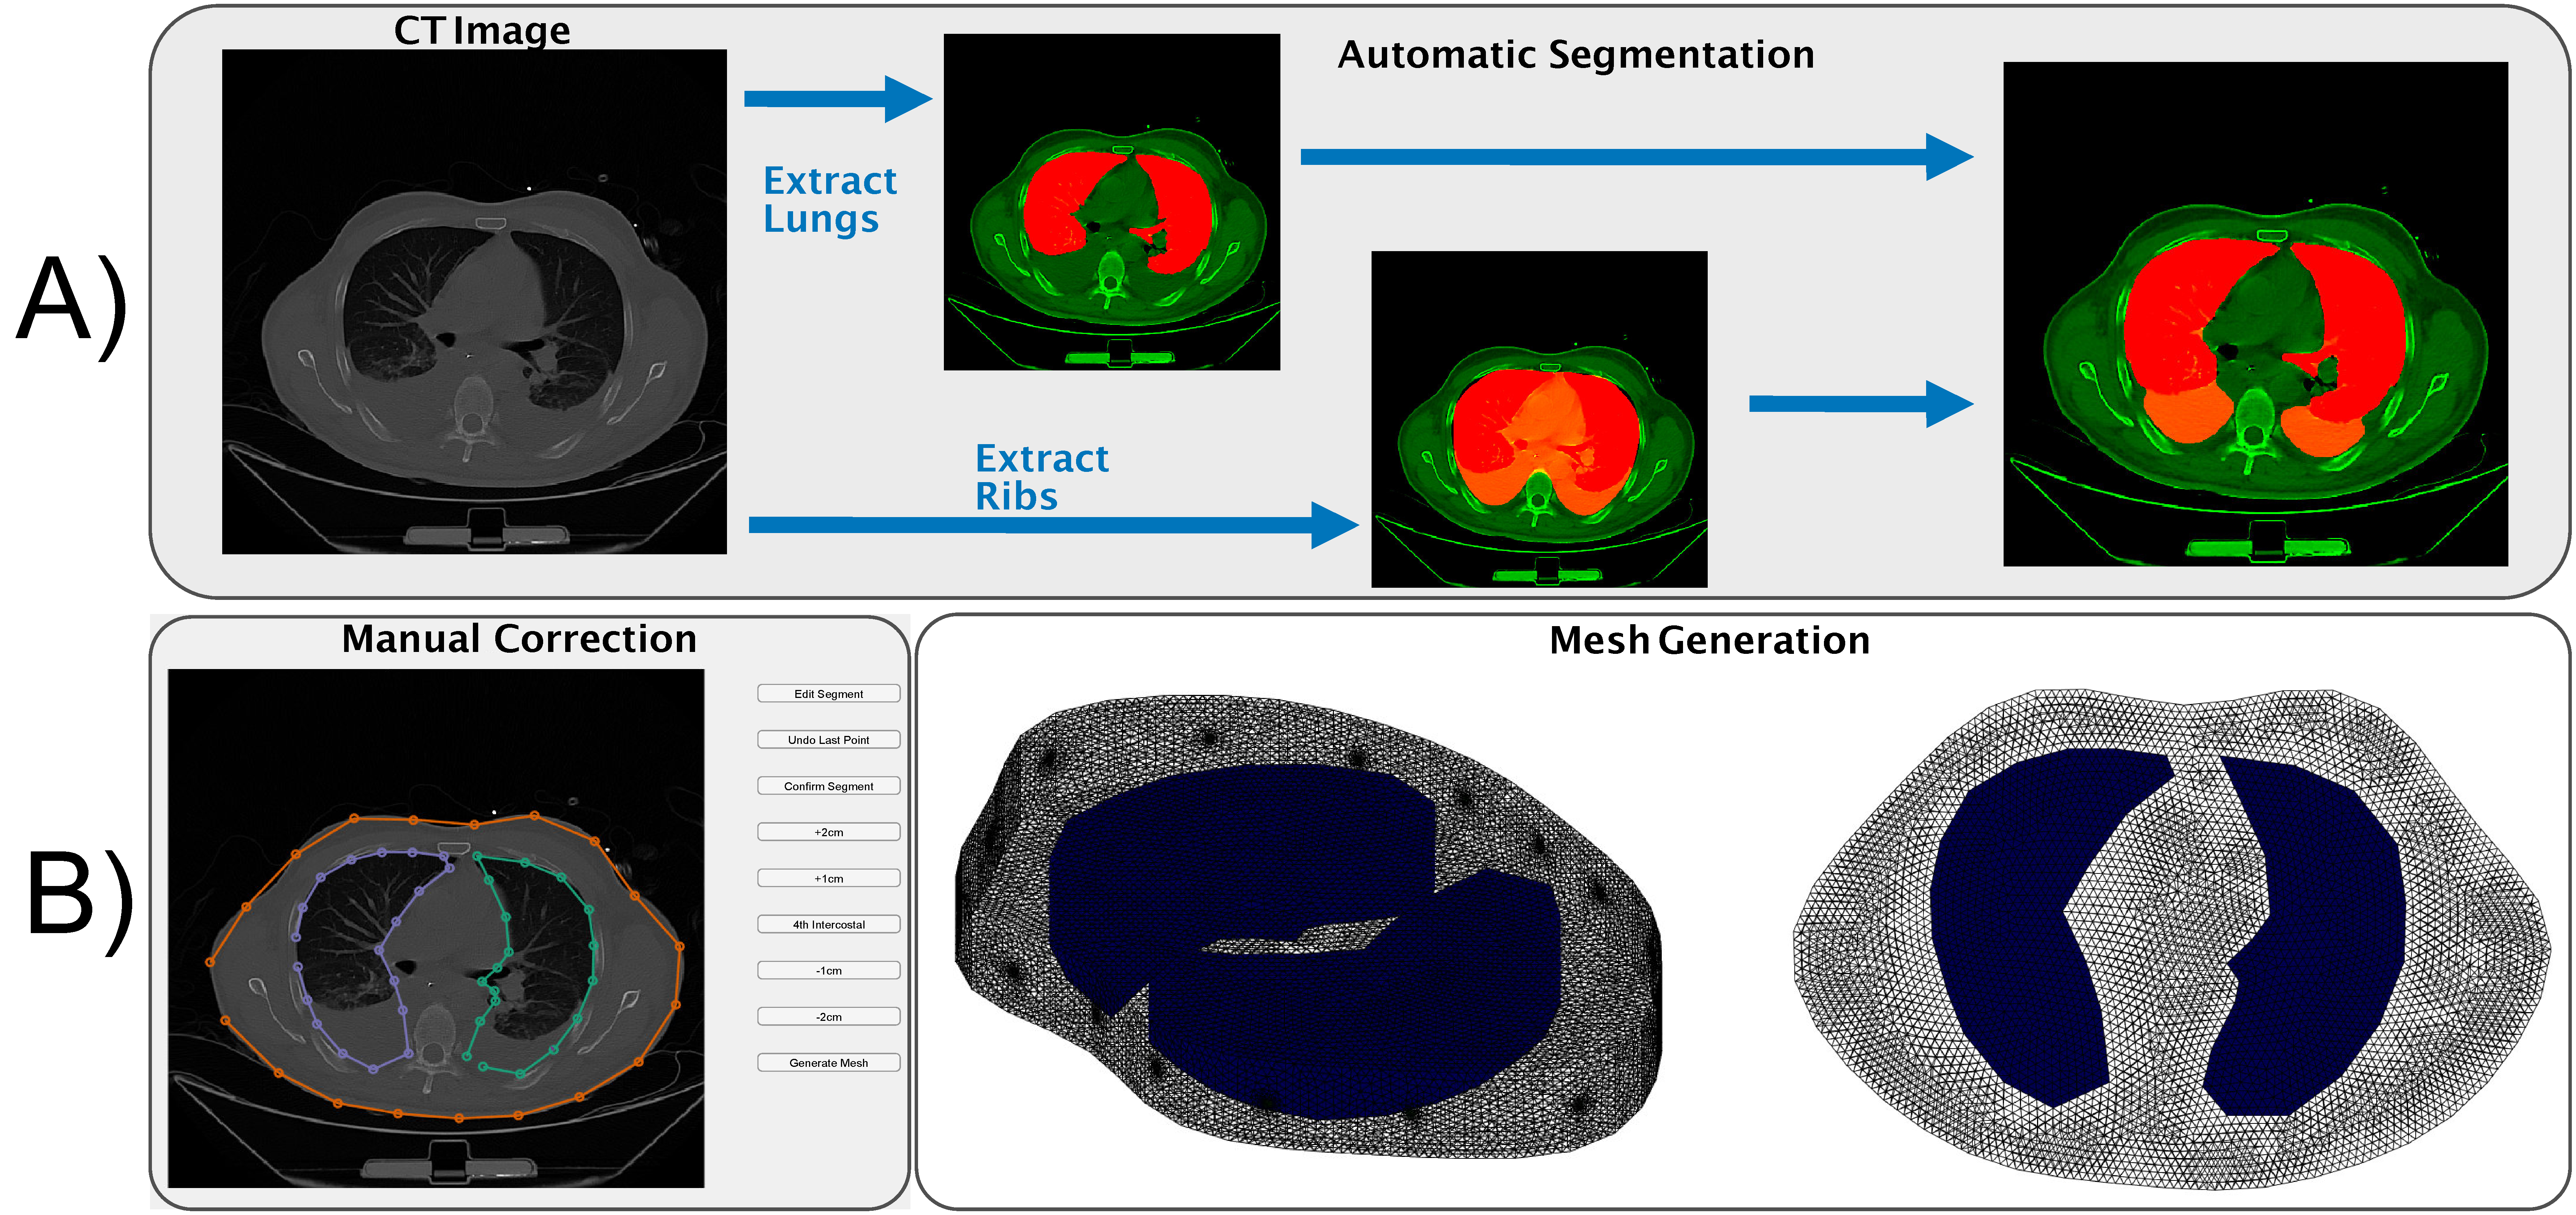
\includegraphics[width=\textwidth]{chapter5-CT_to_mesh/imgs/methods_figure.pdf}
	\caption[Mesh generation method overiew.]{\label{fig:segment_overview}%
	An overview of the segmentation and editing process showing: 
	A) A sample raw CT which was thresholded, scaled and adjusted over several 
	adjacent slices to identify
	the lung regions and an enclosed rib area, and the resulting lung estimate; and
	B) A screen  capture of the manual mesh correction process and 2 views of the generated
	mesh.
	}
\end{figure}

For image segmentation and the manual correction interface
Matlab 2021a (Mathworks, USA) with the image 
processing toolbox was used.
Mesh generation and reconstruction was performed with 
EIDORS 3.10~\parencite{adler_eidors_2017} using Matlab 2019b.
At the time of writing Matlab 2019b was required to 
use some EIDORS functionality, but Matlab 2021a provided some additional 
features that improved responsiveness of the 
graphical user interface \acrshort{gui}.

\subsection{Automatic segmentation of the thorax} \label{sec:auto-segment}
Automatic segmentation of lung regions in ARDS patients is challenging due to the variability
in lung tissue intensity, and the presence of fluid or collapsed lung regions. 
In some patients the lung regions were not visible in the image and even manual
correction of the segmentation required estimation. 
This automatic technique identifies the chest cavity using several adjacent slices to
locate the ribs.
Even when no lung is visible in the image, this produces a starting point
close to the expected boundary to reduce correction time. 
This tool is designed to segment the true lung boundary as closely as possible to 
simplify manual correction.
If no ribs or lung are detected, elipses are placed within the boundary 
close to the expected lung location that 
can be corrected manually.

The designed automatic segmentation uses a diagnostic CT image 
with the slices corresponding to the 4\textsuperscript{th} intercostal space 
identified. 

To begin segmentation, the user must select the series of CT images they 
wish to segment, and the frame number that corresponds to the 4th intercostal 
space. For the 4 test subjects the 4\textsuperscript{th} 
intercostal space was identified manually using
3D Slicer 4~\parencite{fedorov_3d_2012}, as the space between the
4\textsuperscript{th} and 5\textsuperscript{th} ribs underneath the arm.
This location corresponded to the electrode belt placement for EIT measurements.

A detailed algorithmic outline of the automatic segmentation process is 
presented in \fref{app:appendix-algos}.

\subsubsection{External boundary} \label{sec:ext_seg}
The boundary segmentaiton steps are shown in \fref{fig:ext_seg_methods}.
To segment the boundary, the selected raw CT slice 
(A in \fref{fig:ext_seg_methods}) 
was adjusted so that the
intensity of the lung tissue was 0 and the maximum image value was 1 
(B in \fref{fig:ext_seg_methods}). 
Next the image was eroded and reconstructed 
to remove small features and retain large structures 
(C in \fref{fig:ext_seg_methods}).
Finally the image was binarized (D in \fref{fig:ext_seg_methods}),
and holes were filled (E in \fref{fig:ext_seg_methods}), 
to give the final boundary (F in \fref{fig:ext_seg_methods}).

\begin{figure}
	\centering
	% Use the following line with your images (pdf preferred)
	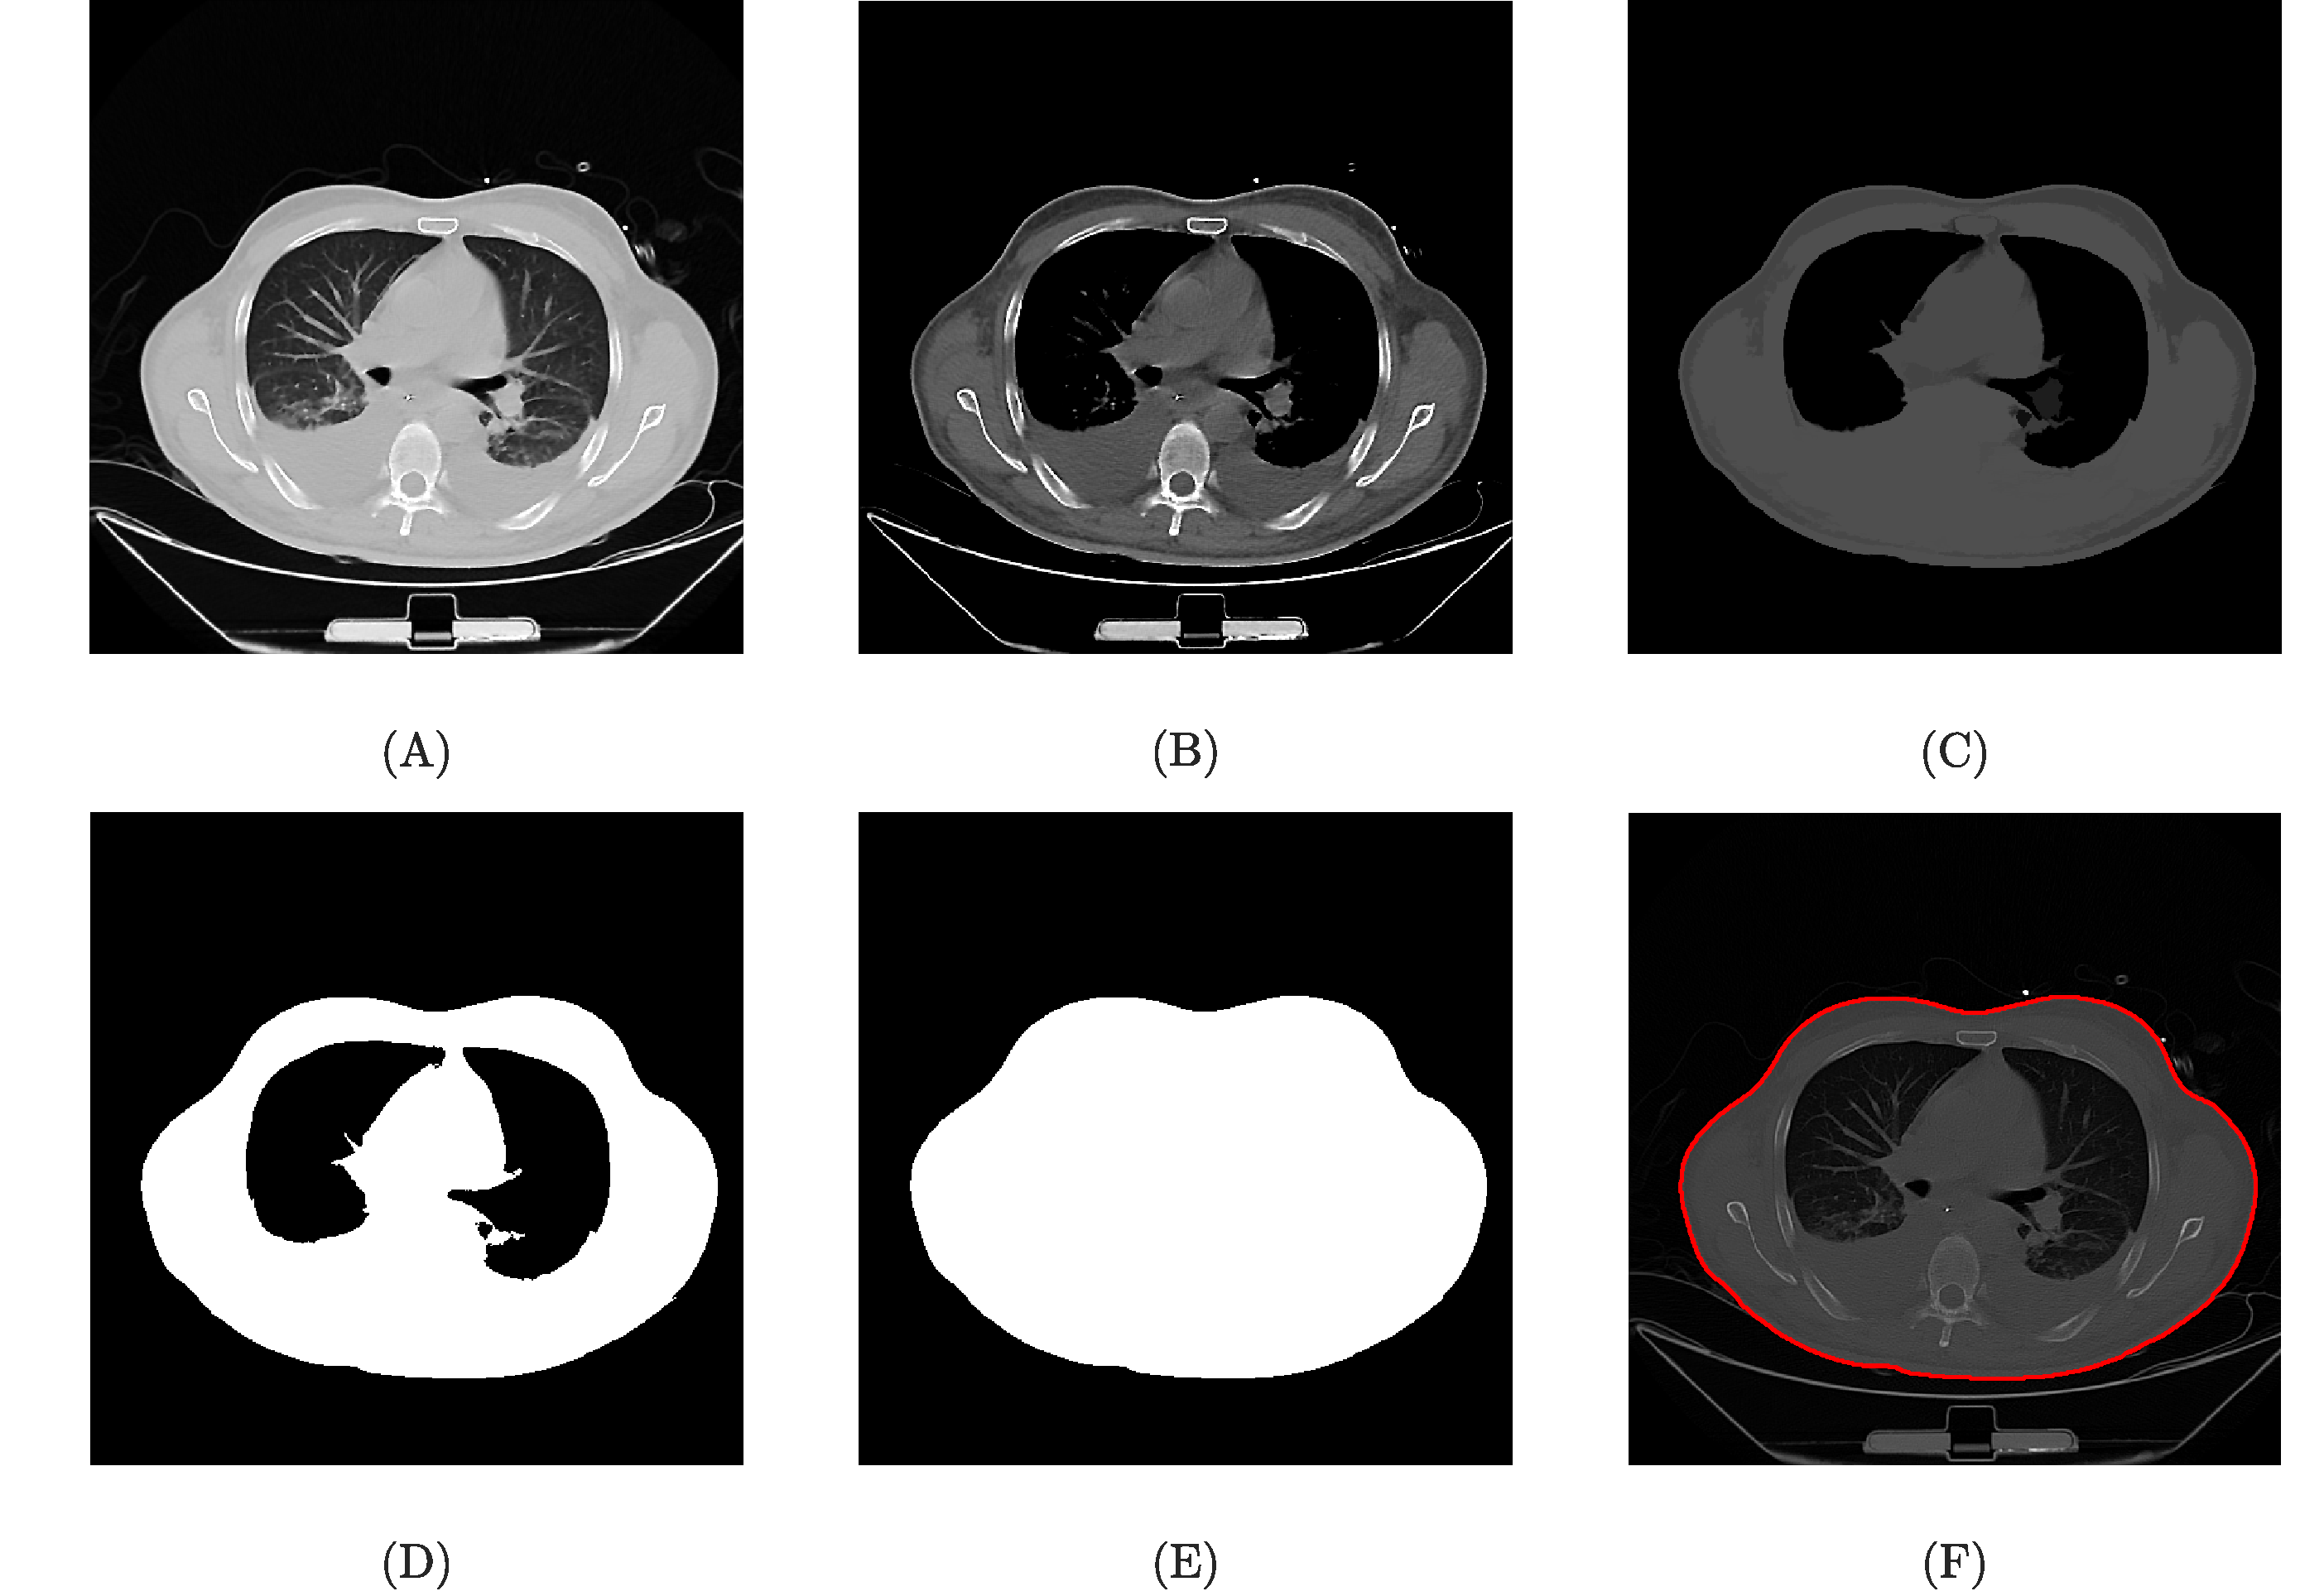
\includegraphics[width=\textwidth]{chapter5-CT_to_mesh/imgs/boundary_seg_methods.pdf}
	\caption[Boundary segmentation methods.]{\label{fig:ext_seg_methods}%
	A raw CT iamge of the 4th intercostal slice (A) 
	was adjusted based on the lung density (B), 
	eroded and reconstructed (C), then binarized (D) and 
	filled to give the final boundary (F).
	}
\end{figure}

\subsubsection{Chest cavity}
To segment the chest cavity 7 slices above and below the 4\textsuperscript{th}
intercostal space were used giving 15 slices to segment. 
To begin, the external boundary of the selected slice was
used (segmented using the method in \fref{sec:ext_seg}). 
The initial boundary 
(A in \fref{fig:cav_seg_methods})
was eroded to form a mask from the shrunken boundary shape
(B in \fref{fig:cav_seg_methods}).
This mask was used on a binarized image to extract bones and bright objects from
within the thorax 
(C in \fref{fig:cav_seg_methods}).
The image was closed to fill  holes and identify bones
(D in \fref{fig:cav_seg_methods}).
Next all 15 adjacent slices were superimposed to combine all rib locations
that occured in more than one slice
(E in \fref{fig:cav_seg_methods}).
To fill holes in the ribcage, a rectangular 
elelement with a height of 5 and width of 50 was used to close 
the top half of the image
(F in \fref{fig:cav_seg_methods}).
A final thickening operation was performed to ensure continuity
(G in \fref{fig:cav_seg_methods}).
All objects connected to the boundary were removed 
to give the final chest cavity segmentation
(H in \fref{fig:cav_seg_methods}).

\begin{figure}
	\centering
	% Use the following line with your images (pdf preferred)
	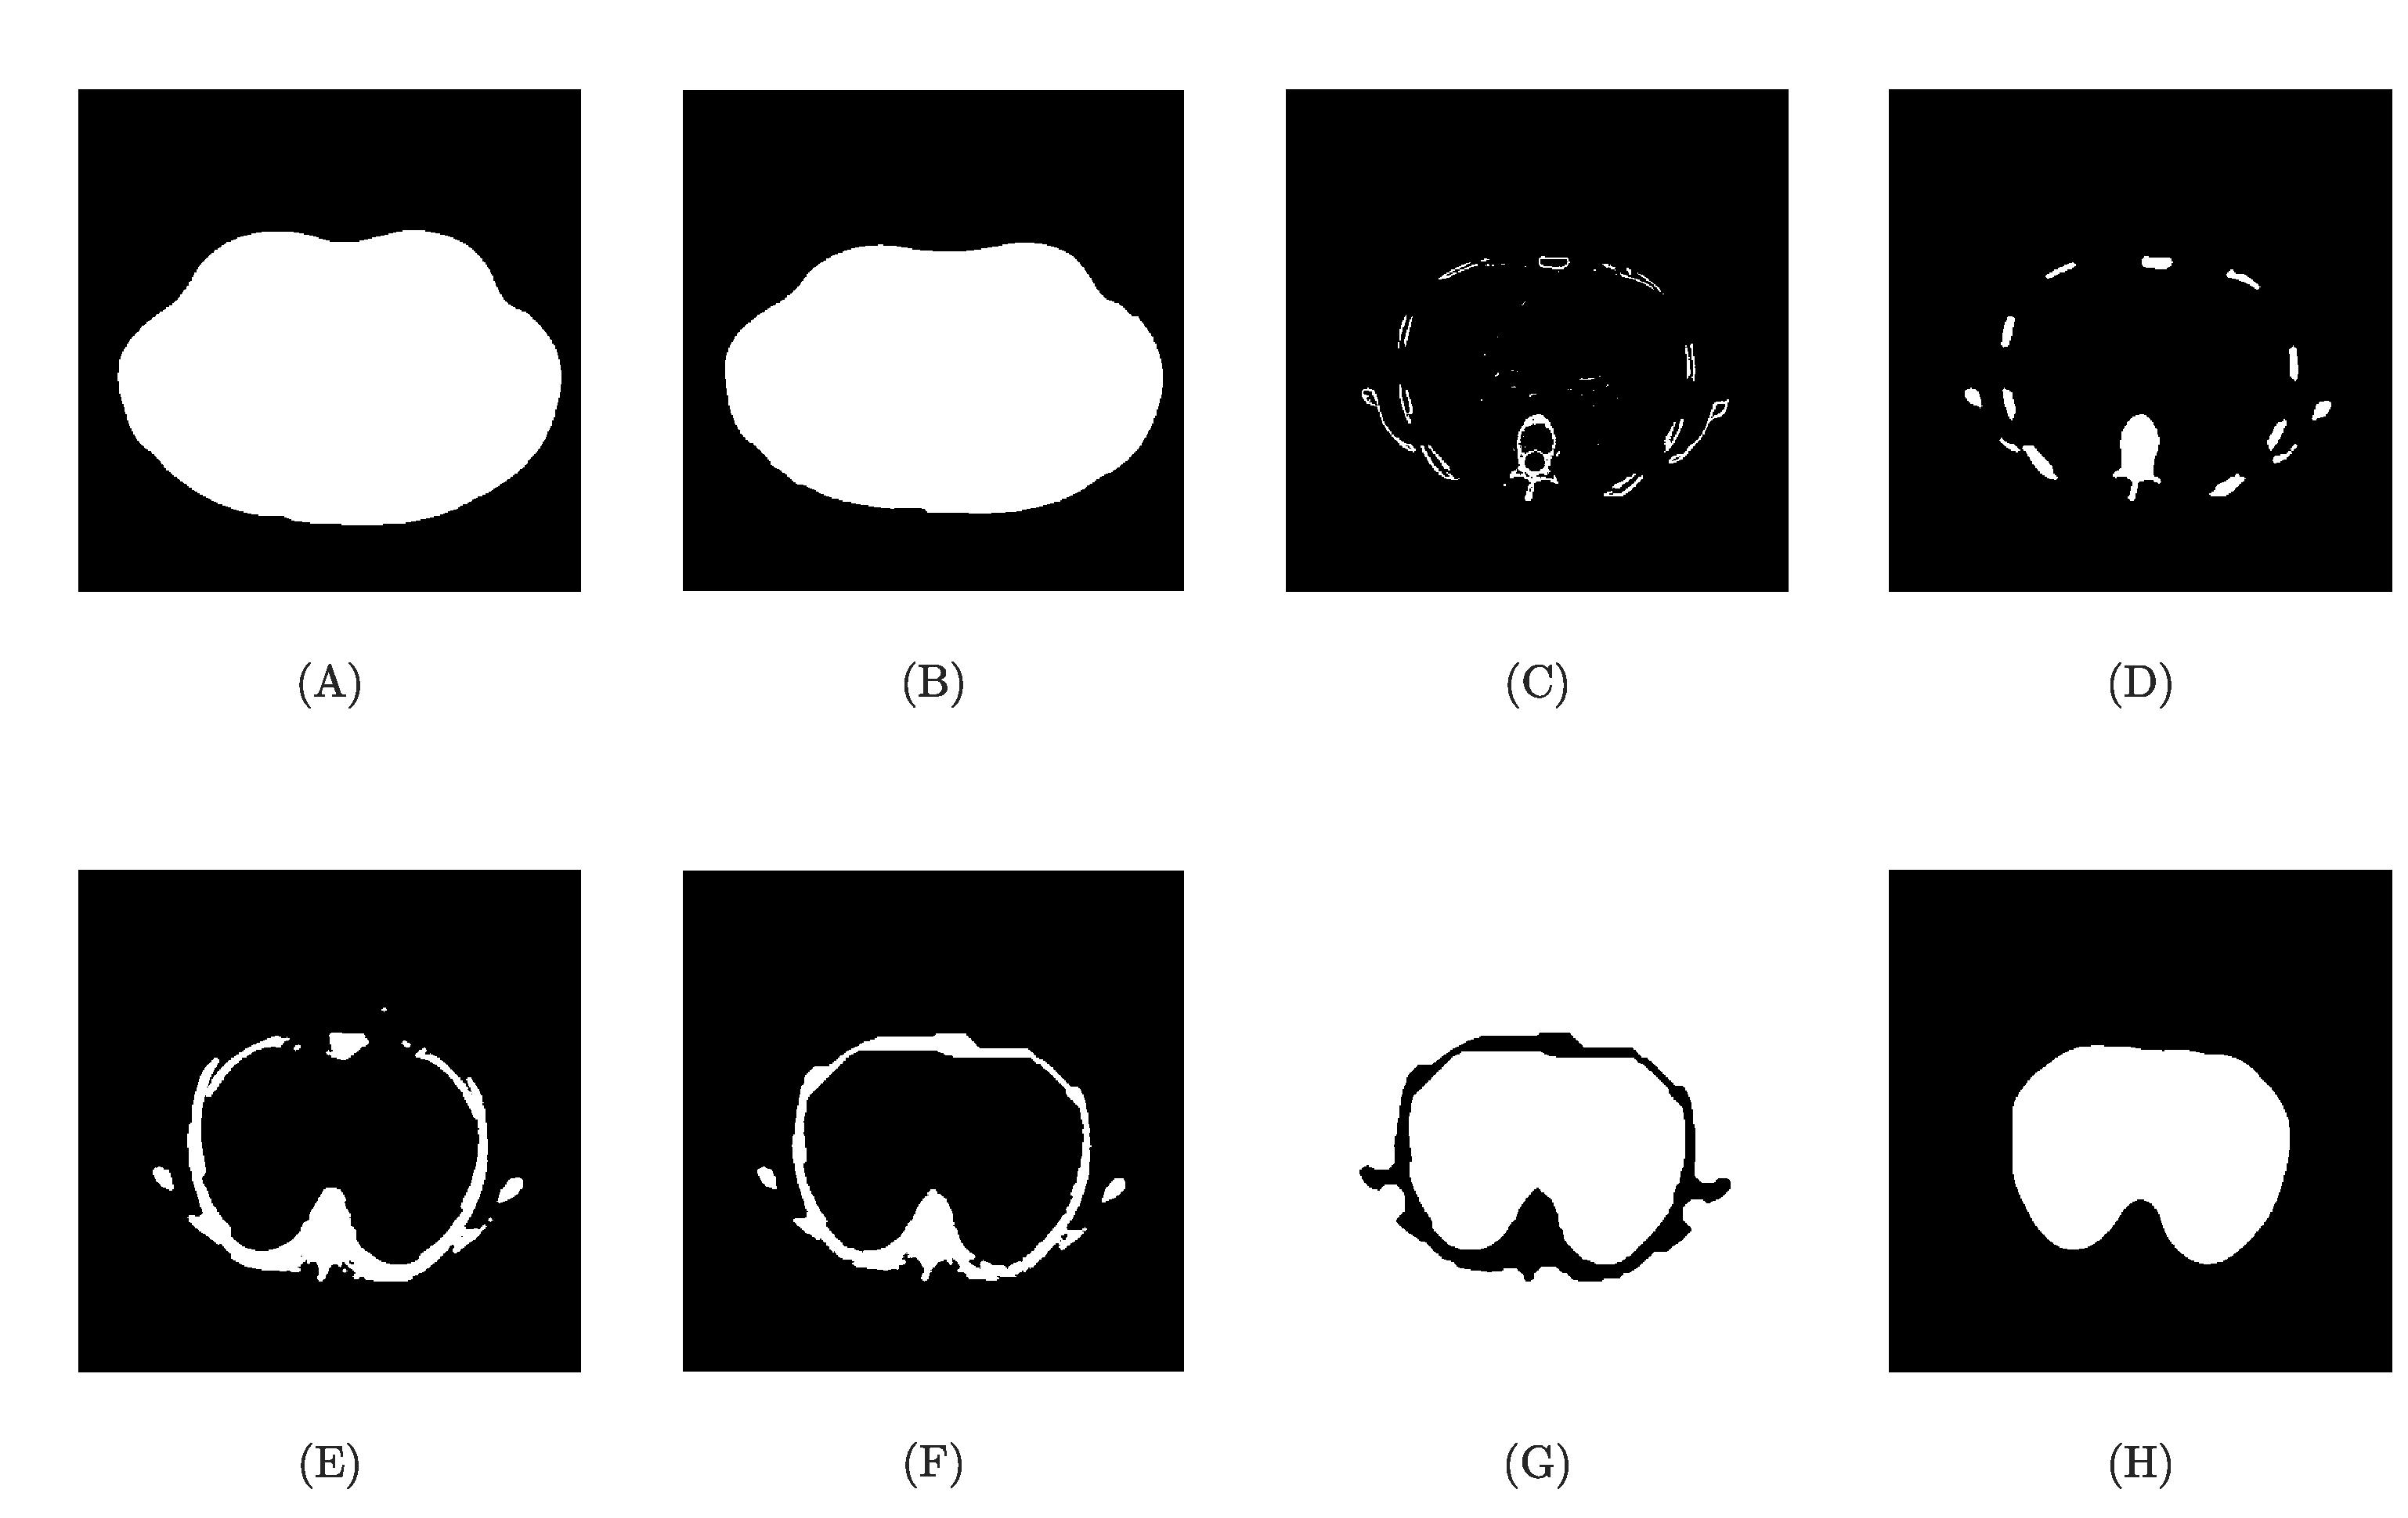
\includegraphics[width=\textwidth]{chapter5-CT_to_mesh/imgs/chest_cavity_seg_methods.pdf}
	\caption[Chest cavity segmentation methods.]{\label{fig:cav_seg_methods}%
	For each of the 15 selected slices the initial external boundary (A)
	was eroded to form a mask from the shrunken boundary shape
	(B). This mask was used on a binarized image to extract bones and bright objects from
	within the thorax (C). The image was closed to fill  holes and identify bones
	(D). Next all 15 adjacent slices were superimposed to combine all rib locations
	that occured in more than one slice (E).
	To fill holes, a rectangular elelement with a height of 5 and width of 50 was used to close 
	the top half of the image (F).
	A final thickening operation was performed to ensure continuity
	(G). All objects connected to the boundary were removed 
	to give the final chest cavity segmentation (H).
	}
\end{figure}


\subsubsection{Lungs}
The lung segmentation was required to work in patients with ARDS and give 
an approximate lung boundary when the lungs were potentially collapsed or filled with 
fluid. To achieve this, a rough lung estimate based on the chest cavity  
was used together with a segmentation of the 
ventilated lung.
The ventilated and non-ventilated regions of the lung were segmented based 
on the chest cavity segmentation (A in \fref{fig:lung_seg_methods}).
First an estimation of the lung region was made by placing an elipse
in the center of the chest cavity segmentation at the thinnest central
point (B in \fref{fig:lung_seg_methods}). Next a ventilated lung estimate 
(C in \fref{fig:lung_seg_methods})
was made
by inverting the binarized image from the external boundary segmentation
(D in \fref{fig:ext_seg_methods}). 
Finally a complete lung estimate was generated by removing any part of the
simple lung estimate (B in \fref{fig:lung_seg_methods}) that was within 5 
pixels of the ventilated lung estimate, and combining the two 
lung estimates with a closing operation. 
This was able to give a close estimate of the lung boundary even in cases where
little or no lung tissue was visually distinguishable. 

\begin{figure}
	\centering
	% Use the following line with your images (pdf preferred)
	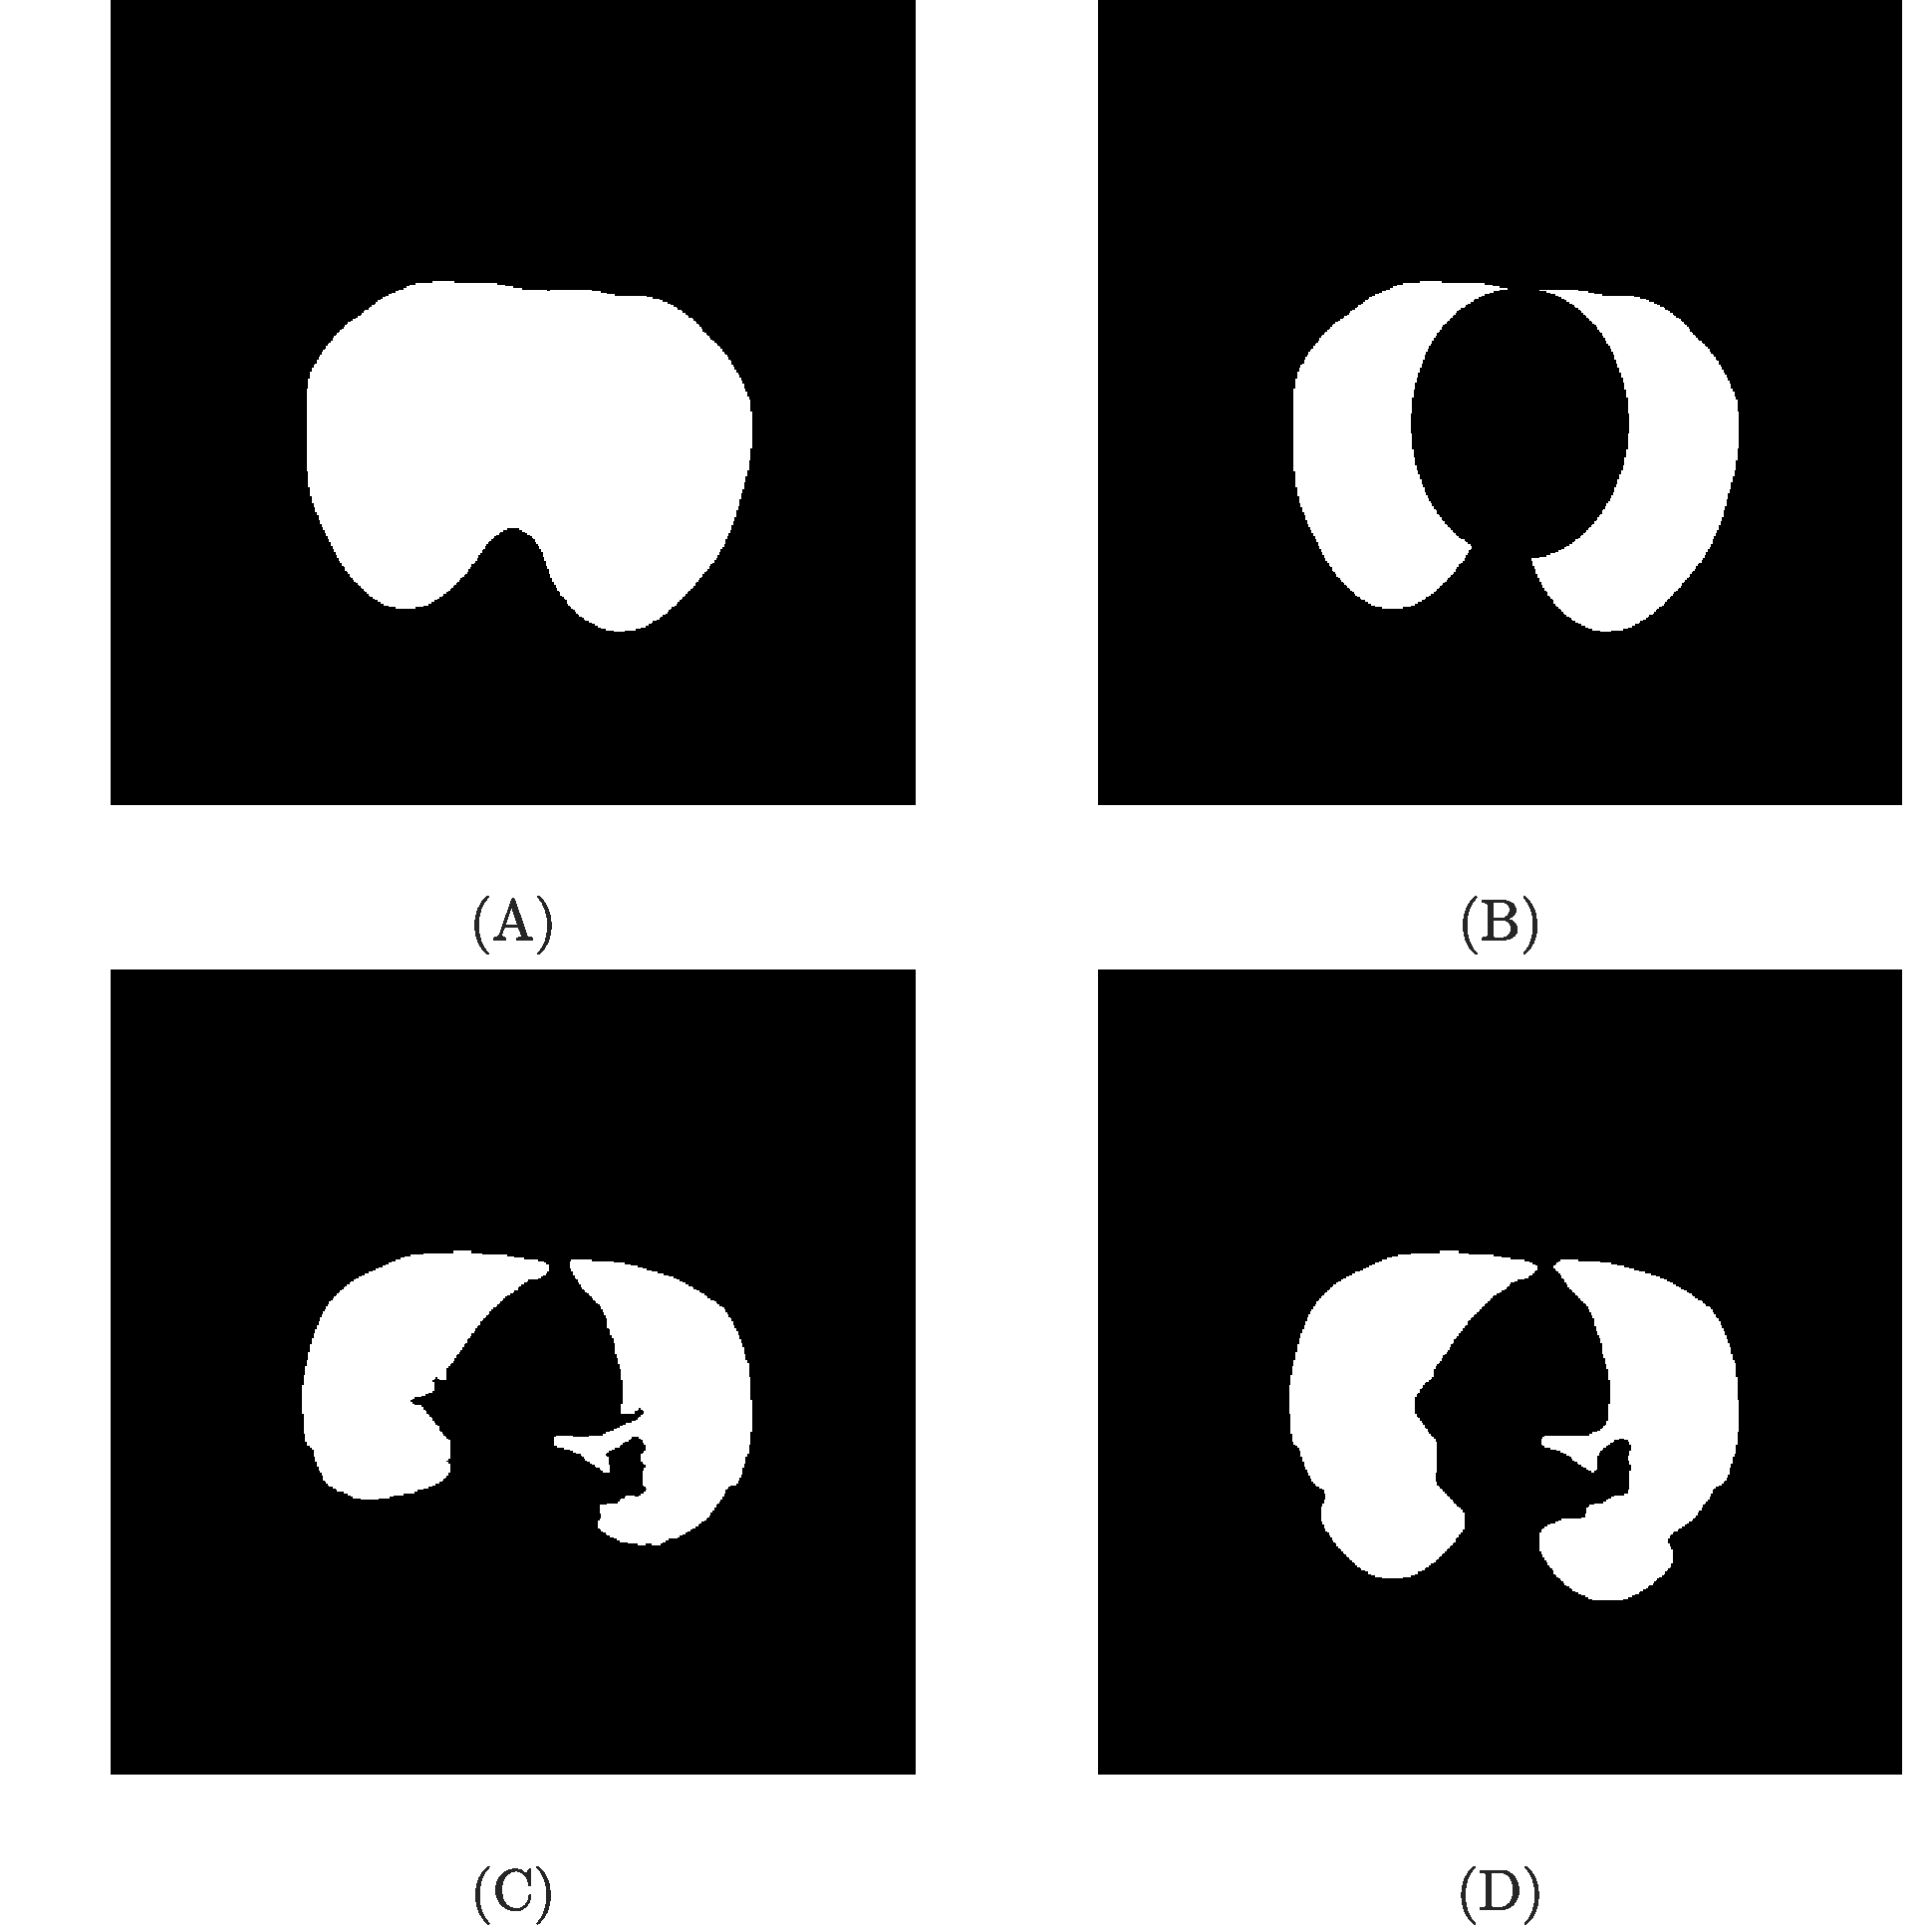
\includegraphics[width=\textwidth]{chapter5-CT_to_mesh/imgs/lung_seg_methods.pdf}
	\caption[Lung segmentation methods.]{\label{fig:lung_seg_methods}%
	An approximation of the lung boundary was generated using the chest cavity segmentaiton
	(A) with an elipse to remove the heart region (B).
	This was combined with a segmentation of the ventilated lung region (C) 
	to give a total lung estimate (D).
	}
\end{figure}

\subsection{Manual segmentation correction}  \label{sec:correct-segment}
Although the automatic segmentation was carefully designed to accurately segment the 
lungs, there were often cases where manual correction was required. To ensure accurate
models were generated, an interface for manual correction was created. 
This tool allowed the user to correct the boundry for a selected CT slice. 
20 points of the segmented boundary for each of the lungs and the external 
boundary were used for correction and placed over 
the corresponding CT image slice.

The segmentation correction tool was designed to save the segmentation with information
on the selected image squence and frame of the 4\textsuperscript{th} intercostal space 
for reference. 
The segmentation correction also allowed users to load and correct previously saved
segmentations, or overwrite them completely.
An example of the setup, and available input for the segmentation 
correction GUI is shown in \fref{fig:seg_load}.
To make segmentation simpler, all data such as the frame of the 4\textsuperscript{th}
intercostal space was saved after the inital load stage. Even if the segmentation 
was not completed the user did not have to re-enter patient details the next 
time the same CT series was loaded. 
An option was also added to manually add an adjustment value for the automatic
segmentation of the ribs if now ribs were detected during automatic segmentation. 
This was not needed as the ribs were sucessfully identified in all test patients.
The software was also designed to have informative error messages for segmentation 
errors for the user to troubleshoot, letting the user know that no ribs or no lungs 
were detected. 

\begin{figure}
	\centering
	% Use the following line with your images (pdf preferred)
	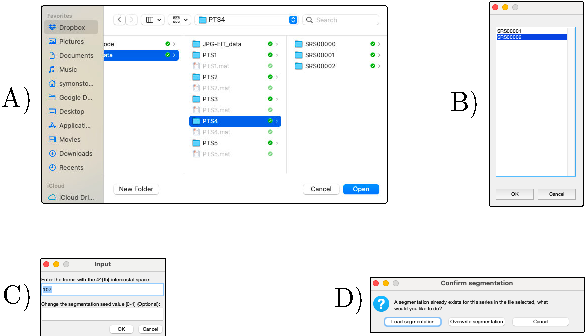
\includegraphics[width=\textwidth]{chapter5-CT_to_mesh/imgs/SegmentationAppSetup.pdf}
	\caption[Manual segmentation data loading]{\label{fig:seg_load}%
	The data loading stages for the manual segmentation program arer shown.
	A) A folder of patient data is selected. B) The desired CT data series is selected.
	C) The inital segmentation frame of the 4\textsuperscript{th} intercostal space 
	is loaded from the patient settings file or input by the user. Optinoally an 
	adjustment to the inidial segmentation thresholding value can be input if the 
	segmentation steps failed to locate ribs in the CT image. D) If an existing,
	manually corrected segmenation was saved, the user is asked before a new segmentaion 
	is made.
	}
\end{figure}

If an error was made during manual correction the user could undo
the last change or revert the selected point to the original location. 
Keyboard shortcuts were assigned to each of the functions to reduce the time required
to segment each slice.

\Fref{fig:seg-app-loaded} shows an example of the matlab GUI for manually correcting
the automatic segmentation. To segment the user would click \emph{Edit Segment} 
then select and move each point that required correction. The first click by the user
selected the nearest point, and the subsequent click placed the point at the new location. 
The slice to be corrected could be selected, the finished segmentation could
be saved, and a mesh could be generated. 

\begin{figure}
	\centering
	% Use the following line with your images (pdf preferred)
	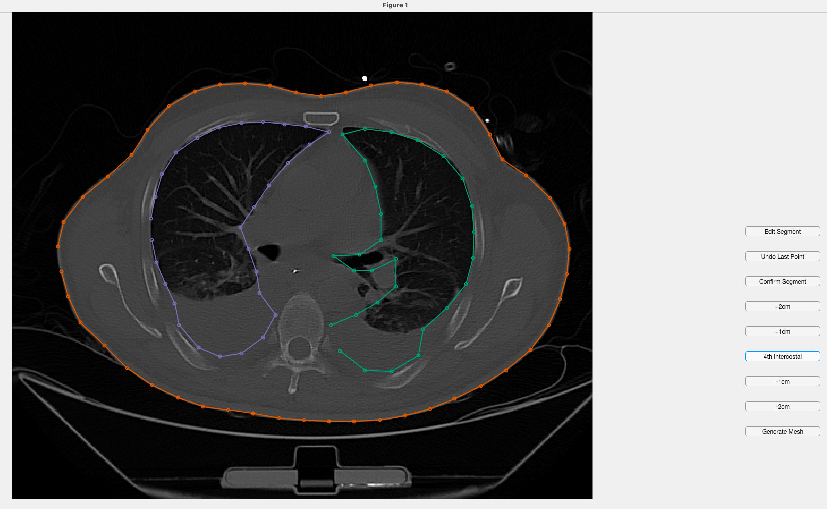
\includegraphics[width=\textwidth]{chapter5-CT_to_mesh/imgs/SegmentationAppLoaded.pdf}
	\caption[Manual segmentation interface with initial input]{\label{fig:seg-app-loaded}%
	An example of a segmentation after being loaded into the segment editor program. 
	The buttons on the right show the optons available to the user, and the left shows the 
	CT image for the corresponding slice with the automatic segmentation overlayed.
	}
\end{figure}

After moving each point an arrow was drawn between the original and new location of the
point last moved to indicate the change and allow the user to see if the
placement was correct. An example of a corrected slice showing the arrow to indicate
a point had been moved is shown in \fref{fig:seg-app-corrected}.

\begin{figure}
	\centering
	% Use the following line with your images (pdf preferred)
	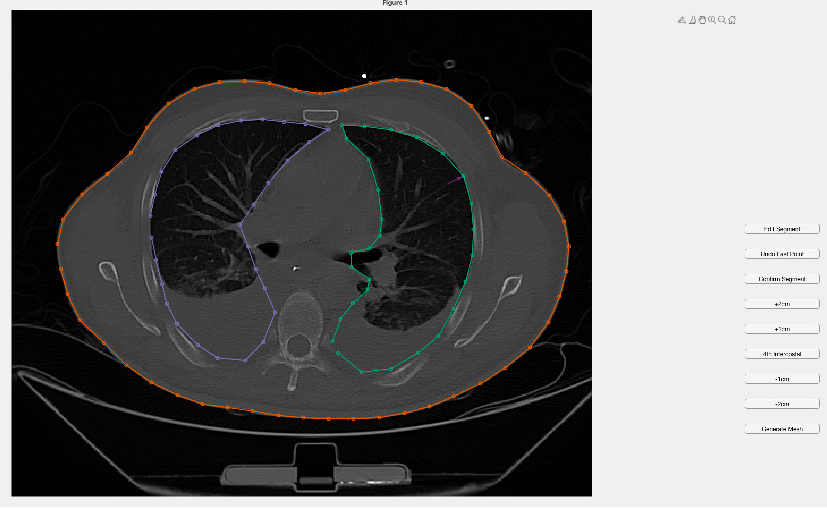
\includegraphics[width=\textwidth]{chapter5-CT_to_mesh/imgs/SegmentationAppCorrected.pdf}
	\caption[Manually corrected segmentation]{\label{fig:seg-app-corrected}%
	An example of a manually corrected segmentation with the arrow indicating the initial
	and new location of the last moved point. The selected point was moved for illusrtative
	purposes and was not based on the initial segmentation.}
\end{figure}

The end result was a GUI that allowed for quick correction of the automatic segmentation 
results. Spatial information from the DICOM image was also saved so that meshes could be
designed to have the correct diameter and be correctly configured to the patient size.
The final option allowed the used to generate the mesh. 

\subsection{Mesh generation} \label{sec:mesh-gen}
There is currently no available tool to automatically generate 3D meshes for 
EIT image reconstruction from a set of points, so the model was simplified using an
an extrusion techniqe for the boundary from the 4\textsuperscript{th} intercostal space. 
The \verb!mk_extruded_model! 
function~\parencite{grychtol_fem_2013}
in EIDORS v3.10~\parencite{adler_eidors_2017} was used to extrude the boundary 
of a single segmenation to a height of 20 cm.
The  lungs were specified 2 ways, the first method used extruded 2D lungs, 
from the single segmentation, and the second generated a 3D lung from several segmented
slices of the lungs. 
To do this an alphashape was created using all points in the 
lung segmentation and the elements of the mesh from the corresponding region 
were selected as the lung. 

To generate a generic mesh for comparison the \verb!mk_library_model! function in 
EIDORS was used which has available geometry for a cylindrical model with lung regions
and a genertic model of a human thorax.

All images were reconstructed using GREIT for 2D
imaging ~\parencite{adler_greit_2009}. For the GREIT 
reconstructions the noise figure was set to 0.5, 
500 targets with a radius of 5cm were used for training.

\subsection{Evaluation on ARDS patients} \label{sec:gi-scores}

Diagnostic CT data was acquired from 4 male patients aged 39--74. 
All patients were diagnosed with ARDS.

EIT data were recorded on all patients
with a 2D arrangement of 16 electrodes placed at the 
4\textsuperscript{th} intercostal space using the 
Draeger EIT system. 
All patients were on mechanical ventilation
at the time of recordings, but the exact 
ventilation parameters are unknown.

To evaluate the effect of the custom models on GI index, 
the scores were computed on 
the generic male model and the custom EIT model generated 
using the segmentation tool.

The GI index was calculated using the method
presented by Zhao et al.~\cite{zhao_evaluation_2009} 
using the lung regions from the 
forward model. 
An estimate of ventilated lung area ($A_V$) relative to the 
total lung area was calculated from the CT images  
by dividing the area of the total lung over the ventilated
lung area 
(\fref{eq:ventilated_lung_est}).
\begin{equation}\label{eq:ventilated_lung_est}
	A_V = \frac{A_{\text{ventilated lung}}}{A_{\text{total lung}}}
\end{equation}

This was used to determine if the calculated index
followed the same trend as the percentage of total lung
that was ventilated in the CT image.

\section{Results}

The goal of the automatic segfmentation algorithm was to 
generate segmentaions that were accurate for quick 
and easy manual correction. \Fref{fig:lung-seg-results}
shows the result of the automatic segmentation regions.
the red overlay indicates the healthy lung segmentation,
and the orange overlay indicated regions that were added
using the estimation method. 
The lungs were examined viually to determine 
how much manual correction was required. During testing
we found that the level of accuracy was sufficient to 
complete segmentation correction for each subject in 
under 1 minute.

\begin{figure}
	\centering
	% Use the following line with your images (pdf preferred)
	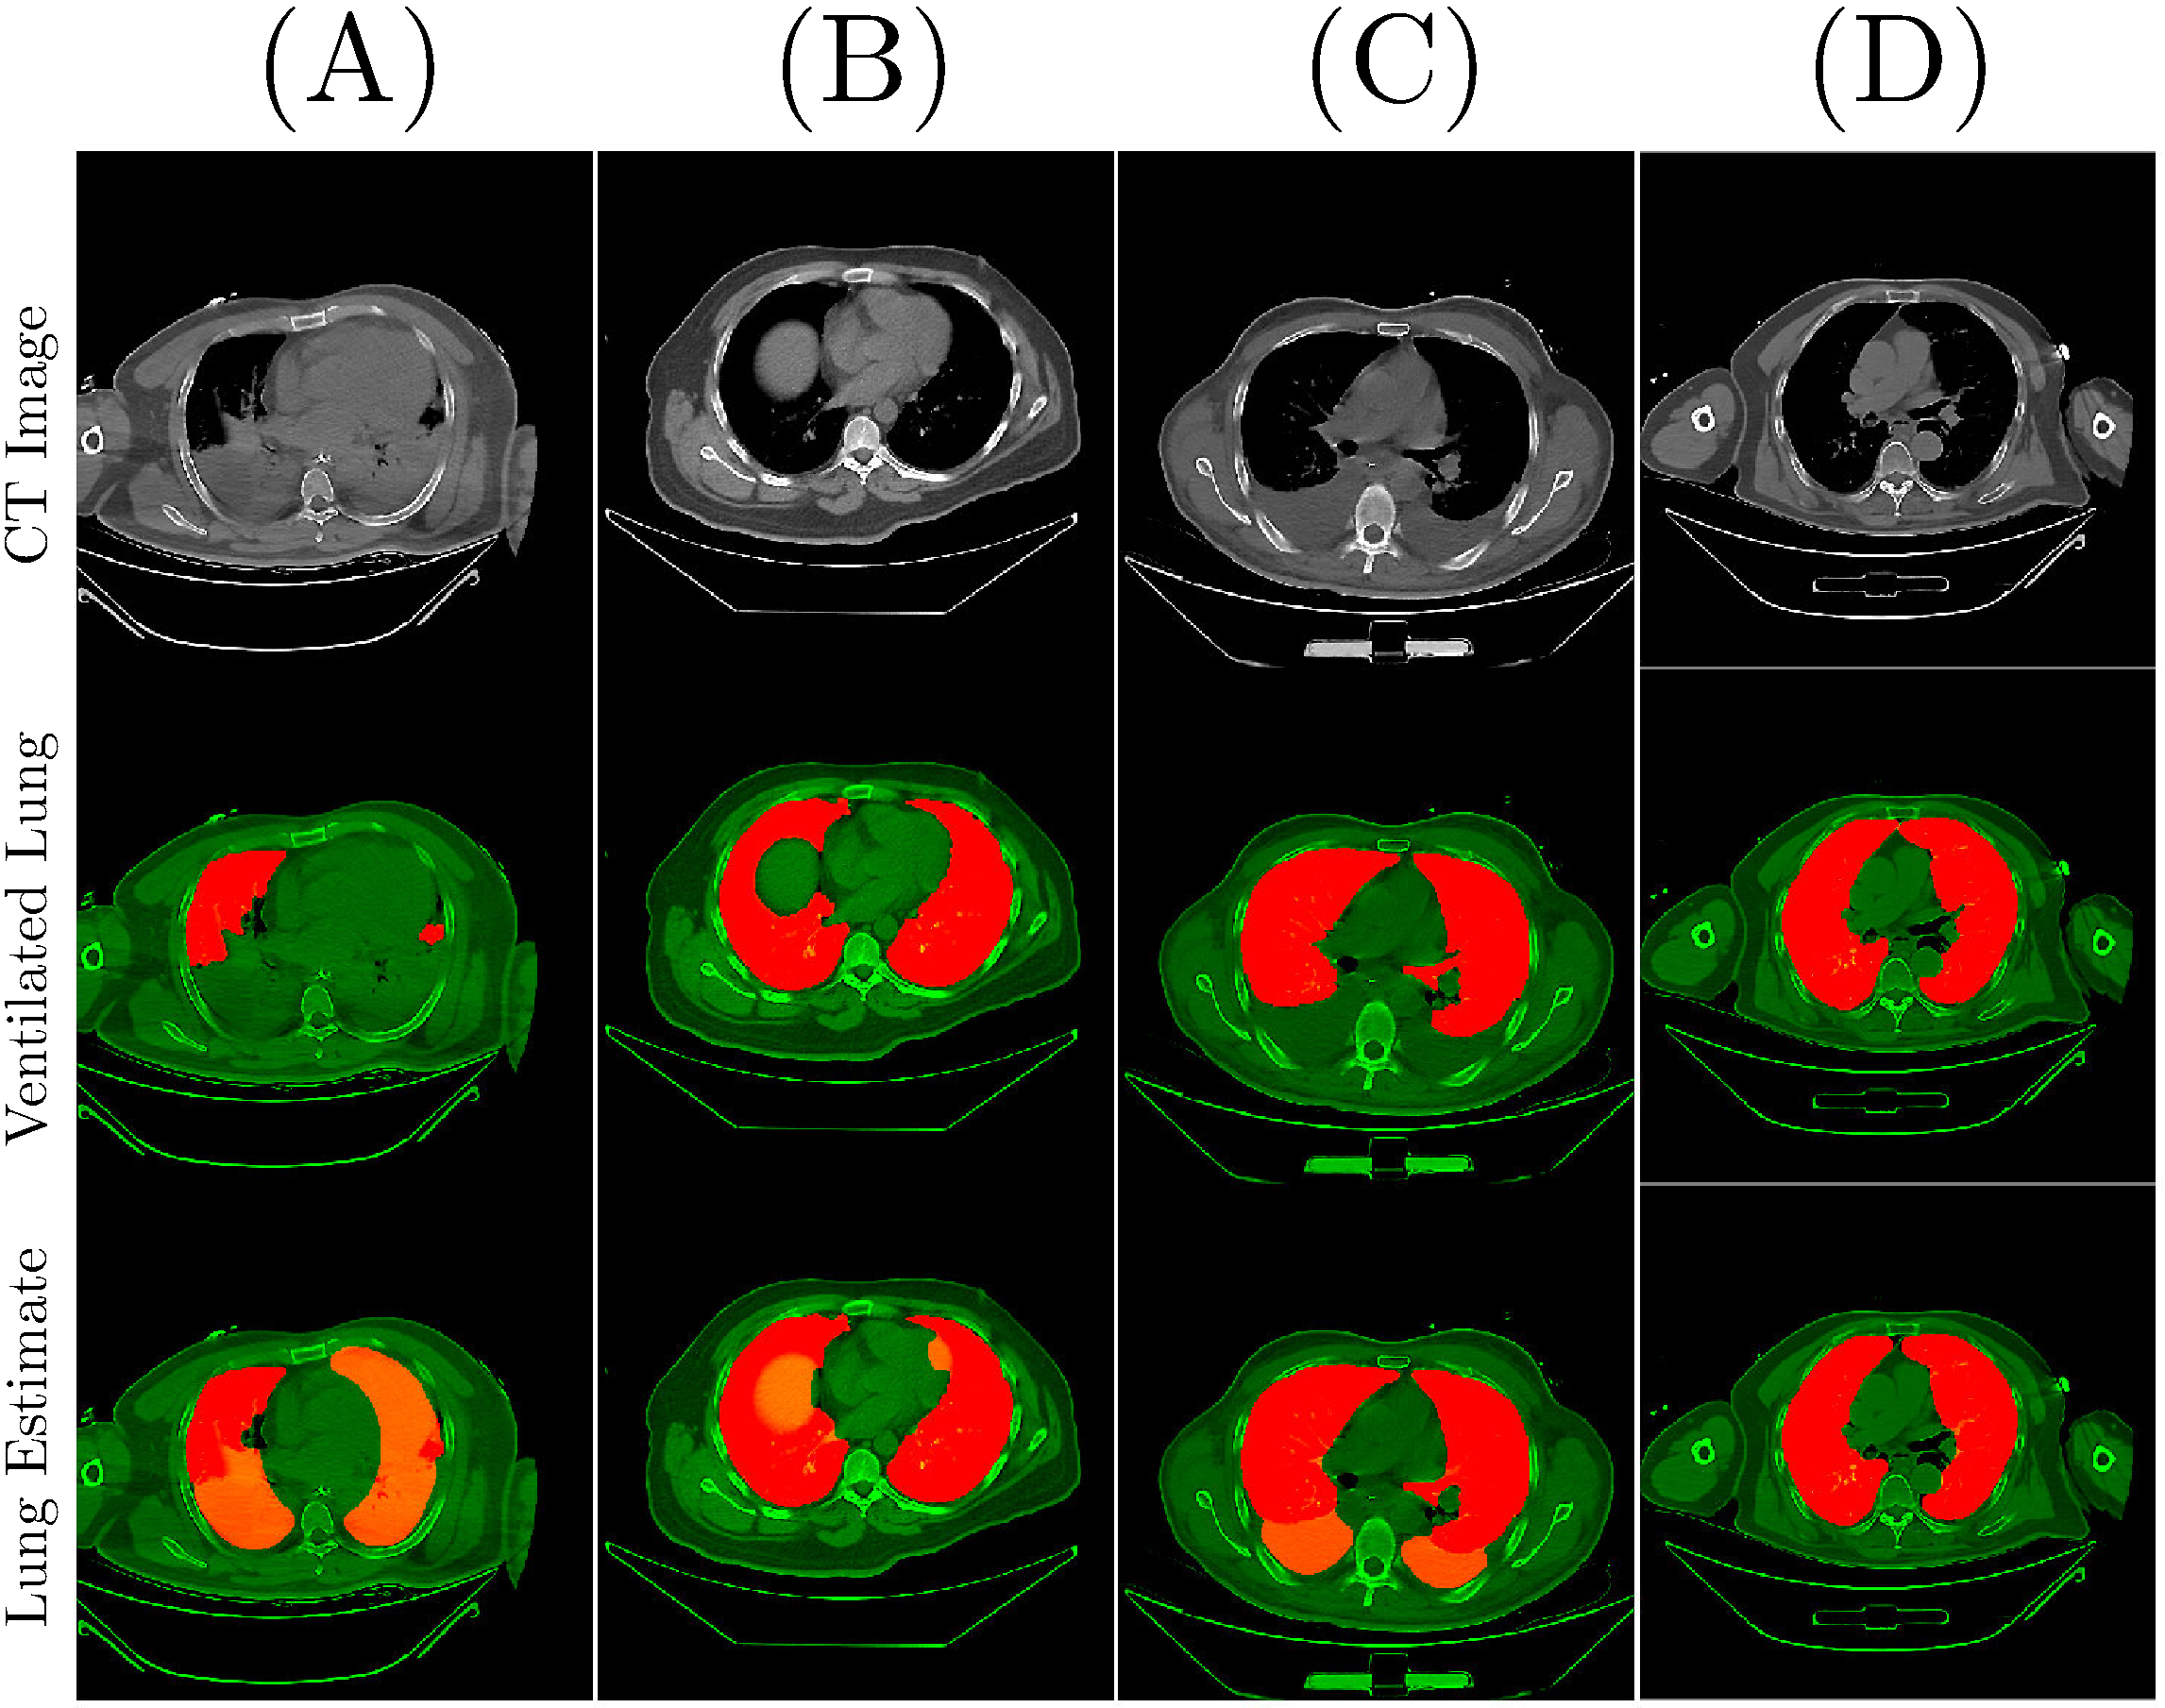
\includegraphics[width=\textwidth]{chapter5-CT_to_mesh/imgs/lung_segmentation_results.pdf}
	\caption[Lung segmentation results]{\label{fig:lung-seg-results}%
	This figure shows the results of the automatic segmentation algorithm. The letters A--D 
	represent the 4 patients. Patient A had a significant portion of the lung that was not
	ventilated, so an estimate was required to obtain lung regions. The ventilated lung estimate
	is shown in red on the 2\textsuperscript{nd} and 3\textsuperscript{rd} colums.
	The total lung area using the chest cavity and ventilated lung area is shown in the
	bottom row.}
\end{figure}

The segmentaiton results show that there is good identification of the
ventilated lung region from the automatic segmentation. The estimated lung regions also helped to 
give starting approximations for the lungs and decrease required manual 
correction time when there was limited ventilated lung in the available CT image.

Sample meshes generated from the segmented images are shown in \fref{fig:fem-results} 
for subect C (in \fref{fig:lung-seg-results}).

\begin{figure}
	\centering
	% Use the following line with your images (pdf preferred)
	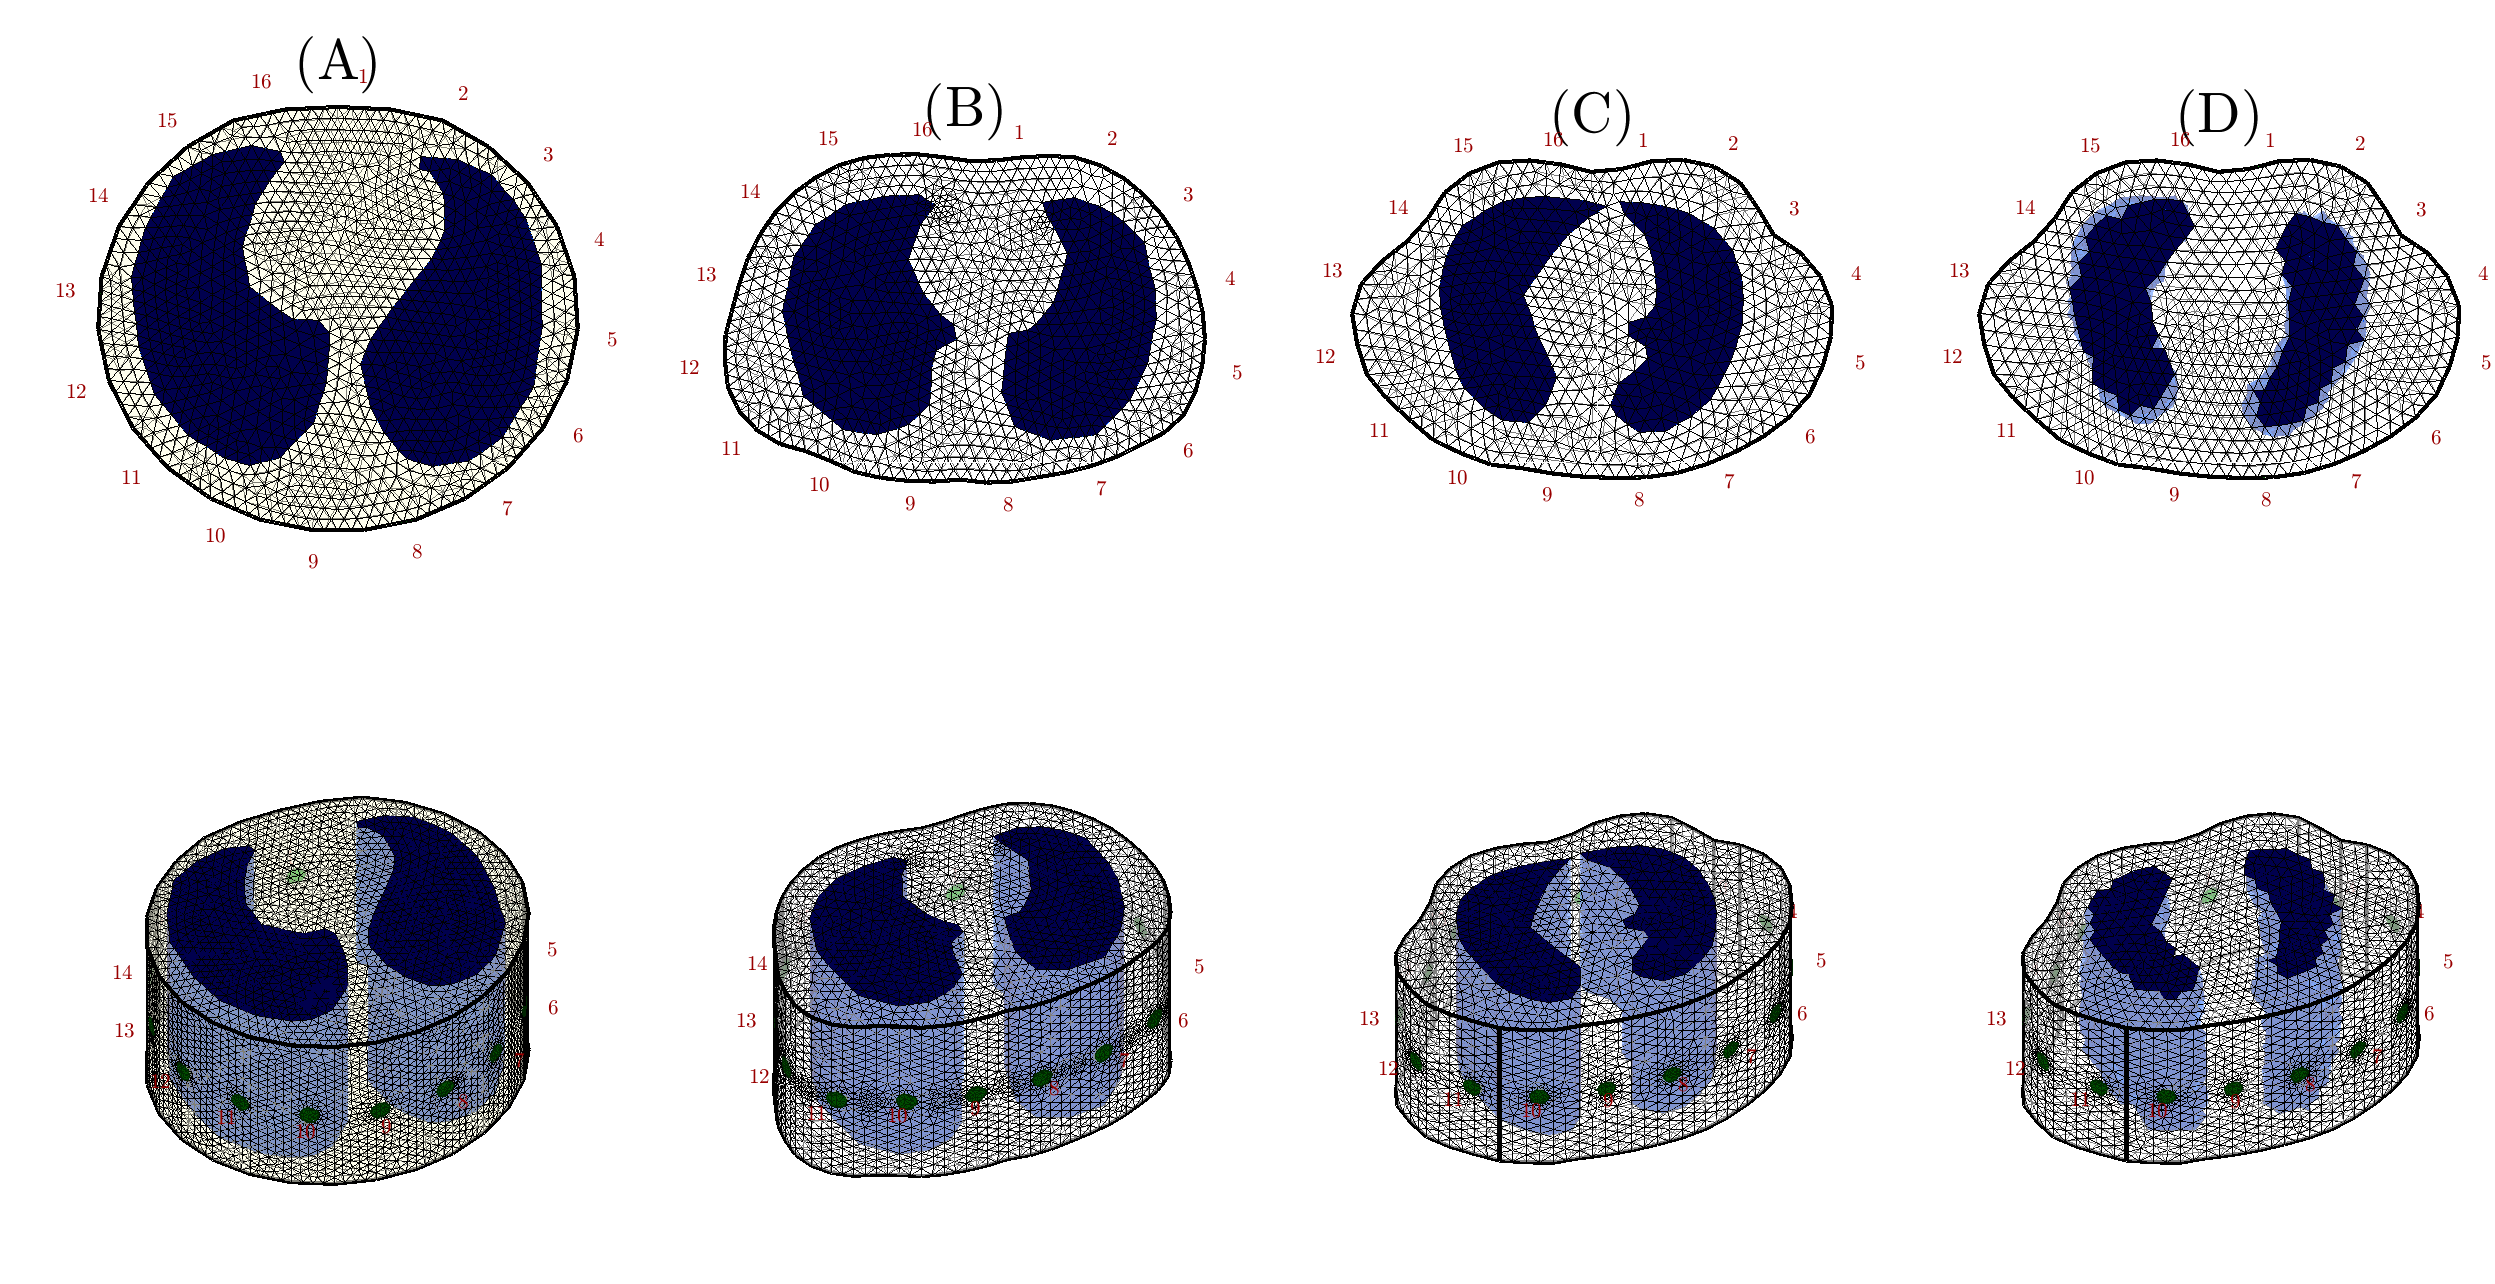
\includegraphics[width=\textwidth]{chapter5-CT_to_mesh/imgs/fem_models_PT04.pdf}
	\caption[]{\label{fig:fem-results}%
	example meshes and electrode locations for subject B (from \fref{fig:lung-seg-results}).
	Model (A) is circular with lung regions. Model (B) uses the generic chest model from EIDORS 
	and models (C) and (D) use the custom segmentation boundaries. Model (C) uses 2D lung boundaries 
	from the 4th intersoctal space extruded for the model height. Model (D) selects all elements
	are within the 3D lung boundary identified by the segmentation results.
	}
\end{figure}









Data from 4 ARDS patients with CT
and EIT were used to develop a segmentation 
and correction tool to identify 
the lungs and boundary of the body.  
Segmentation was done using the 4th intercostal space, 
with 10 adjacent CT 
slices to form an enclosed chest cavity. 
The lungs
and exterior boundary were identified by increasing the contrast
and identifying an appropriate threshold.
Each segmentation was downsampled to
20 points that could be edited by the user in Matlab. The 
mesh was generated using 
\verb!ng_mk_extruded_model!~\cite{Grychtol2012} in EIDORS 
3.10~\cite{Adler2019}. Images were reconstructed 
using GREIT~\cite{Adler2009}. 


\begin{figure}
\centering
% Use the following line with your images (pdf preferred)
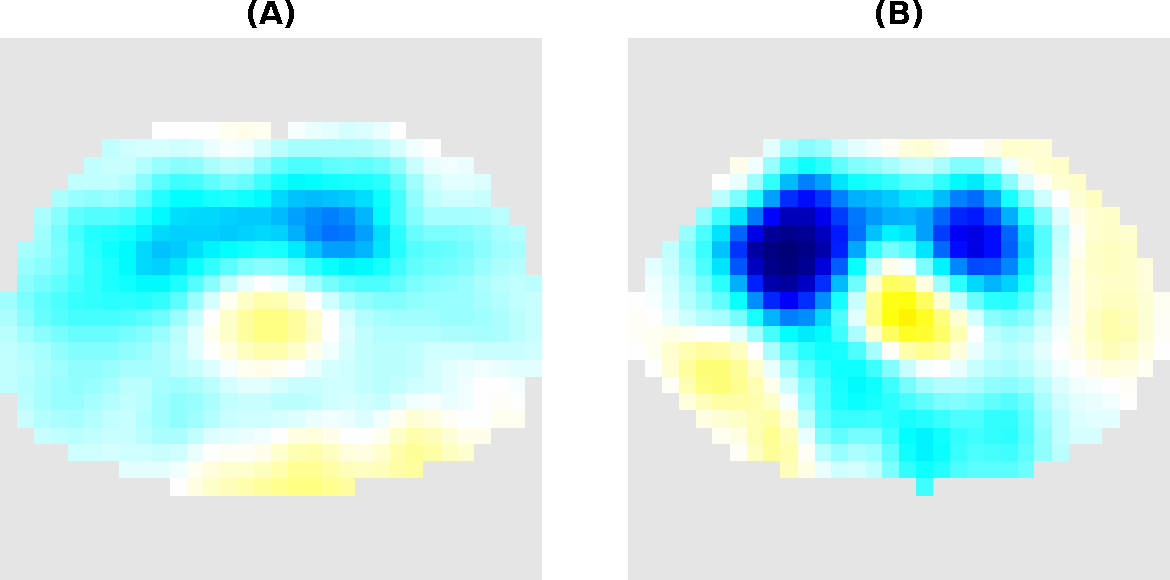
\includegraphics[width=\textwidth]{chapter5-CT_to_mesh/imgs/basic_vs_advanced_3_cropped.pdf}
\caption{\label{fig:ct_mesh_breath}%
Single breath using: A) generic model B) custom model
}
\end{figure}

Results in figure~\fref{fig:breath} show a reconstructed image 
with more separable lungs in the enhanced model, and a mean GI index for each breath in the 
1 minute 
recording that follows 
trend of the ventilated lung percentage in table~\ref{tbl:twocol}.

\begin{table}
  \centering
  \caption{\label{tbl:twocol} %
  Ventilated lung estimate vs. GI index scores.}
  \begin{tabular}{|p{1.2cm}|p{1.5cm}|p{1.8cm}|p{1.7cm}|}
    \hline
  Subject & Ventilated lung (\%) &
  GI (basic model) & GI (custom model) \\ \hline
  1 & 99.9 & 0.353$\pm$0.004& 0.690$\pm$0.005 \\ 
  2 & 85.5 & 0.640$\pm$0.022& 0.771$\pm$0.020  \\
  3 & 79.6 & 0.695$\pm$0.007& 0.857$\pm$0.009  \\
  4 & 27.0 & 0.614$\pm$0.011&  1.81$\pm$0.053 \\\hline
  \end{tabular}
  \vspace{-1em} 
\end{table}

\section{Discussion}

The goal of this chapter was to design a tool to make custom meshes of 

$\sigma$